\begin{frame}{Context Window Problems}
  \begin{itemize}
    \item[\textcolor{red}{$\blacktriangleright$}] Current LLMs have a finite ``context window'':
      \begin{itemize}
        \item \textbf{GPT-3:} 2K tokens
        \item \textbf{GPT-4:} Up to 128K tokens
        \item \textbf{Claude 3.5:} Up to 200K tokens
      \end{itemize}
    \item[\textcolor{red}{$\blacktriangleright$}] \textbf{Problems:}
      \begin{itemize}
        \item Long documents get truncated
        \item Token limit affects reasoning
        \item Difficult to do document-level QA or summarization
      \end{itemize}
  \end{itemize}
\end{frame}

\begin{frame}{Context Window Problems}
  \begin{center}
    \textbf{Example of a Context Window}
    \vspace{1em}

    % A manual diagram in TikZ for a context window on a token sequence.
    % xscale is set so the two span labels fit side by side without colliding.
    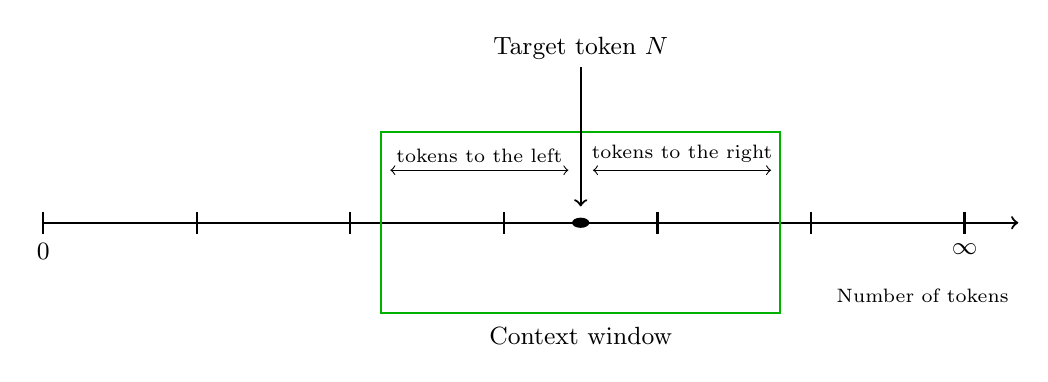
\begin{tikzpicture}[xscale=1.95, yscale=1.15, font=\small]
      % Draw number line
      \draw[->, thick] (0,0) -- (6.35,0);
      % Tick marks and labels
      \foreach \x in {0,1,2,3,4,5,6}
        \draw[thick] (\x,0.12) -- (\x,-0.12);
      \node[below] at (0,-0.12) {0};
      \node[below] at (6,-0.12) {$\infty$};
      \node[anchor=north east, font=\scriptsize] at (6.35,-0.62) {Number of tokens};

      % Draw context window box
      \draw[thick, green!70!black] (2.2,1.0) rectangle (4.8,-1.0);
      \node[below] at (3.5,-1.05) {Context window};

      % Target token N
      \fill (3.5,0) circle (1.6pt);
      \draw[->, thick] (3.5,1.72) -- (3.5,0.18);
      \node[above] at (3.5,1.70) {Target token $N$};

      % Arrows for left/right tokens
      \draw[<->] (2.26,0.58) -- (3.42,0.58);
      \node[above, font=\scriptsize] at (2.84,0.56) {tokens to the left};
      \draw[<->] (3.58,0.58) -- (4.74,0.58);
      \node[above, font=\scriptsize] at (4.16,0.56) {tokens to the right};
    \end{tikzpicture}
  \end{center}
\end{frame}

\begin{frame}{Context Window Problems}
  \begin{center}
    {\large \textbf{Why \textcolor{blue}{Bigger Context Windows} Aren't Always Better?}}
  \end{center}
  \vspace{1em}
  % \parbox width subtracts the frame rule and separation so the boxes stay inside
  % their columns; the fixed height keeps all four aligned top and bottom.
  \begin{columns}[t,onlytextwidth]
    \begin{column}{0.235\textwidth}
      \fcolorbox{red}{white}{%
        \parbox[t][3.1cm][t]{\dimexpr\linewidth-2\fboxsep-2\fboxrule\relax}{%
          \centering
          \textbf{\textcolor{red}{1}}\\[0.3em]
          \textbf{Information Overload}\\[0.4em]
          {\scriptsize
          $\bullet$ Excess data can overwhelm the LLM.\\
          $\bullet$ Reduces focus and slows performance.
          }
        }%
      }%
    \end{column}
    \begin{column}{0.235\textwidth}
      \fcolorbox{orange}{white}{%
        \parbox[t][3.1cm][t]{\dimexpr\linewidth-2\fboxsep-2\fboxrule\relax}{%
          \centering
          \textbf{\textcolor{orange}{2}}\\[0.3em]
          \textbf{Getting Lost in Data}\\[0.4em]
          {\scriptsize
          $\bullet$ Large windows prioritize edges,\\
          $\bullet$ Missing key middle info.
          }
        }%
      }%
    \end{column}
    \begin{column}{0.235\textwidth}
      \fcolorbox{teal}{white}{%
        \parbox[t][3.1cm][t]{\dimexpr\linewidth-2\fboxsep-2\fboxrule\relax}{%
          \centering
          \textbf{\textcolor{teal}{3}}\\[0.3em]
          \textbf{Poor Management}\\[0.4em]
          {\scriptsize
          $\bullet$ More data leads to noise,\\
          $\bullet$ Redundancy, and potential bias.
          }
        }%
      }%
    \end{column}
    \begin{column}{0.235\textwidth}
      \fcolorbox{black}{white}{%
        \parbox[t][3.1cm][t]{\dimexpr\linewidth-2\fboxsep-2\fboxrule\relax}{%
          \centering
          \textbf{4}\\[0.3em]
          \textbf{Long-Range Issues}\\[0.4em]
          {\scriptsize
          $\bullet$ Understanding relationships\\
          becomes harder with large context windows.
          }
        }%
      }%
    \end{column}
  \end{columns}
\end{frame}

\begin{frame}{Context Window Problems}
  \centering
  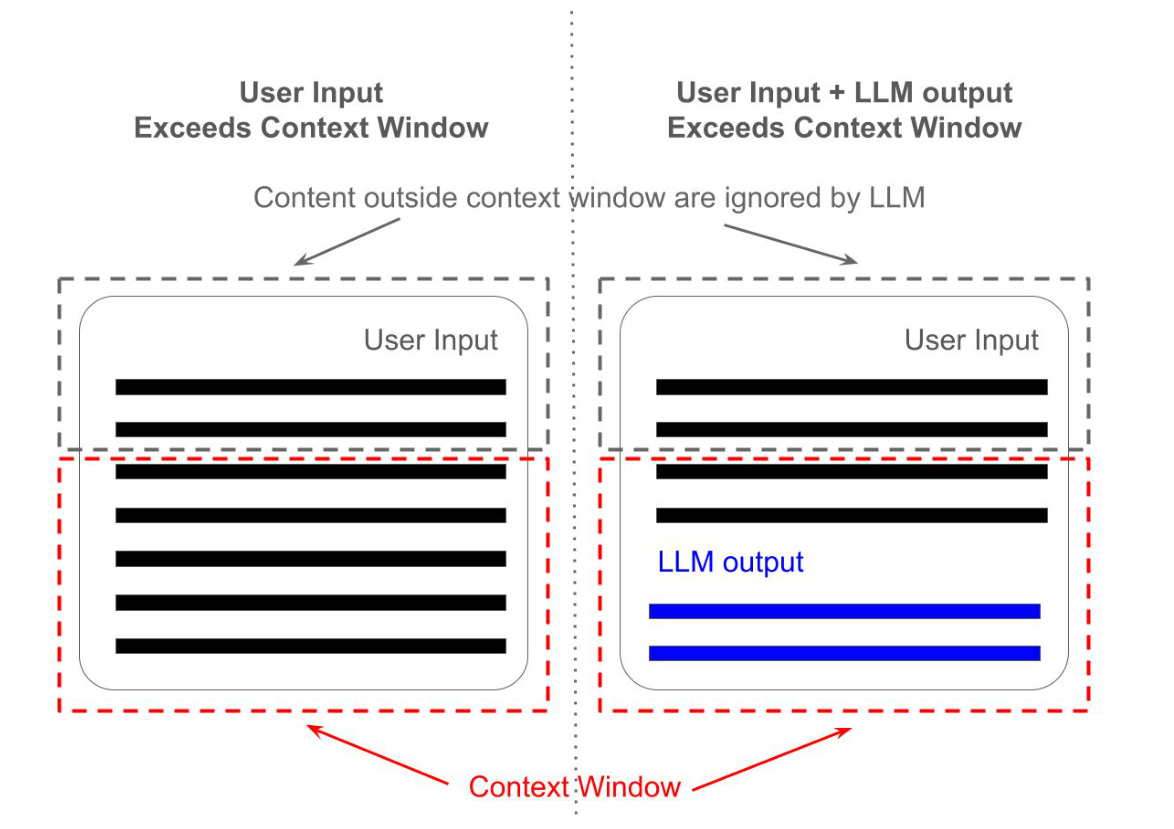
\includegraphics[width=0.60\paperwidth,height=0.60\paperheight,keepaspectratio]{images/large-language-models/llm_context_window_problems.png}

  {\scriptsize Source: ``\href{https://prompt.16x.engineer/blog/chatgpt-context-window-token-limit}{ChatGPT Context Window and Token Limit}'', 16x Prompt blog, 2024.}
\end{frame}
